\section*{Portable abstraction of hierarchical architectures for high-\/performance computing}





 See also \hyperlink{a00379_further_reading}{Further Reading}  for links to more sections about hwloc concepts. 

 \hypertarget{a00379_hwloc_summary}{}\section{hwloc Summary}\label{a00379_hwloc_summary}
hwloc provides command line tools and a C A\+PI to obtain the hierarchical map of key computing elements within a node, such as\+: N\+U\+MA memory nodes, shared caches, processor packages, dies and cores, processing units (logical processors or \char`\"{}threads\char`\"{}) and even I/O devices. hwloc also gathers various attributes such as cache and memory information, and is portable across a variety of different operating systems and platforms.

hwloc primarily aims at helping high-\/performance computing (H\+PC) applications, but is also applicable to any project seeking to exploit code and/or data locality on modern computing platforms.

hwloc supports the following operating systems\+:


\begin{DoxyItemize}
\item Linux (including old kernels not having sysfs topology information, with knowledge of cpusets, Scale\+MP v\+S\+MP support, etc.) on all supported hardware, including Intel Xeon Phi and Numa\+Scale Numa\+Connect. 
\item Solaris (with support for processor sets and logical domains) 
\item A\+IX 
\item Darwin / OS X 
\item Free\+B\+SD and its variants (such as k\+Free\+B\+S\+D/\+G\+NU) 
\item Net\+B\+SD 
\item H\+P-\/\+UX 
\item Microsoft Windows 
\item I\+BM Blue\+Gene/Q Compute Node Kernel (C\+NK) 
\end{DoxyItemize}

Since it uses standard Operating System information, hwloc\textquotesingle{}s support is mostly independant from the processor type (x86, powerpc, ...) and just relies on the Operating System support. The main exception is B\+SD operating systems (Net\+B\+SD, Free\+B\+SD, etc.) because they do not provide support topology information, hence hwloc uses an x86-\/only C\+P\+U\+I\+D-\/based backend (which can be used for other O\+Ses too, see the \hyperlink{a00392}{Components and plugins} section).

To check whether hwloc works on a particular machine, just try to build it and run {\ttfamily lstopo} or {\ttfamily lstopo-\/no-\/graphics}. If some things do not look right (e.\+g. bogus or missing cache information), see \hyperlink{index_bugs}{Questions and Bugs}.

hwloc only reports the number of processors on unsupported operating systems; no topology information is available.

For development and debugging purposes, hwloc also offers the ability to work on \char`\"{}fake\char`\"{} topologies\+:


\begin{DoxyItemize}
\item Symmetrical tree of resources generated from a list of level arities, see \hyperlink{a00389}{Synthetic topologies}. 
\item Remote machine simulation through the gathering of topology as X\+ML files, see \hyperlink{a00388}{Importing and exporting topologies from/to X\+ML files}. 
\end{DoxyItemize}

hwloc can display the topology in a human-\/readable format, either in graphical mode (X11), or by exporting in one of several different formats, including\+: plain text, La\+TeX tikzpicture, P\+DF, P\+NG, and F\+IG (see \hyperlink{a00379_cli_examples}{Command-\/line Examples} below). Note that some of the export formats require additional support libraries.

hwloc offers a programming interface for manipulating topologies and objects. It also brings a powerful C\+PU bitmap A\+PI that is used to describe topology objects location on physical/logical processors. See the \hyperlink{a00379_interface}{Programming Interface} below. It may also be used to binding applications onto certain cores or memory nodes. Several utility programs are also provided to ease command-\/line manipulation of topology objects, binding of processes, and so on.

Perl bindings are available from Bernd Kallies on \href{http://search.cpan.org/~bka/Sys-Hwloc-0.10/}{\tt C\+P\+AN}.

Python bindings are available from Guy Streeter\+: 
\begin{DoxyItemize}
\item \href{http://people.redhat.com/streeter/}{\tt Fedora R\+PM and tarball}. 
\item \href{git://git.fedorahosted.org/python-hwloc.git}{\tt git tree} (\href{http://git.fedorahosted.org/git/python-hwloc.git}{\tt html}). 
\end{DoxyItemize}

 \hypertarget{a00379_hwloc_installation}{}\section{hwloc Installation}\label{a00379_hwloc_installation}
The generic installation procedure for both hwloc and netloc is described in \hyperlink{index_common_installation}{Installation}.

The hwloc command-\/line tool \char`\"{}lstopo\char`\"{} produces human-\/readable topology maps, as mentioned above. It can also export maps to the \char`\"{}fig\char`\"{} file format. Support for P\+DF, Postscript, and P\+NG exporting is provided if the \char`\"{}\+Cairo\char`\"{} development package (usually {\ttfamily cairo-\/devel} or {\ttfamily libcairo2-\/dev}) can be found in \char`\"{}lstopo\char`\"{} when hwloc is configured and build.

The hwloc core may also benefit from the following development packages\+: 
\begin{DoxyItemize}
\item libpciaccess for full I/O device discovery ({\ttfamily libpciaccess-\/devel} or {\ttfamily libpciaccess-\/dev} package). On Linux, P\+CI discovery may still be performed (without vendor/device names) even if libpciaccess cannot be used. 


\item A\+MD or N\+V\+I\+D\+IA Open\+CL implementations for Open\+CL device discovery.  
\item the N\+V\+I\+D\+IA C\+U\+DA Toolkit for C\+U\+DA device discovery. It\textquotesingle{}s installation path may be specified at configure time with {\ttfamily --with-\/cuda=/path/to/cuda}.  
\item the N\+V\+I\+D\+IA Management Library (N\+V\+ML) for N\+V\+ML device discovery. It is included in C\+U\+DA since version 8.\+0. Older N\+V\+ML releases were available within the N\+V\+I\+D\+IA G\+PU Deployment Kit from \href{https://developer.nvidia.com/gpu-deployment-kit}{\tt https\+://developer.\+nvidia.\+com/gpu-\/deployment-\/kit} .  
\item the N\+V-\/\+C\+O\+N\+T\+R\+OL X extension library (N\+V\+Ctrl) for N\+V\+I\+D\+IA display discovery. The relevant development package is usually {\ttfamily lib\+X\+N\+V\+Ctrl-\/devel} or {\ttfamily libxnvctrl-\/dev}. It is also available within nvidia-\/settings from \href{ftp://download.nvidia.com/XFree86/nvidia-settings/}{\tt ftp\+://download.\+nvidia.\+com/\+X\+Free86/nvidia-\/settings/} and \href{https://github.com/NVIDIA/nvidia-settings/}{\tt https\+://github.\+com/\+N\+V\+I\+D\+I\+A/nvidia-\/settings/} .  
\item the A\+MD R\+O\+Cm S\+MI library for R\+S\+MI device discovery. The relevant development package is usually {\ttfamily rocm-\/smi-\/lib64} or {\ttfamily librocm-\/smi-\/dev}.  
\item libxml2 for full X\+ML import/export support (otherwise, the internal minimalistic parser will only be able to import X\+ML files that were exported by the same hwloc release). See \hyperlink{a00388}{Importing and exporting topologies from/to X\+ML files} for details. The relevant development package is usually {\ttfamily libxml2-\/devel} or {\ttfamily libxml2-\/dev}.  
\item libudev on Linux for easier discovery of OS device information (otherwise hwloc will try to manually parse udev raw files). The relevant development package is usually {\ttfamily libudev-\/devel} or {\ttfamily libudev-\/dev}.  
\item libtool\textquotesingle{}s ltdl library for dynamic plugin loading if the native dlopen cannot be used. The relevant development package is usually {\ttfamily libtool-\/ltdl-\/devel} or {\ttfamily libltdl-\/dev}.  
\end{DoxyItemize}

P\+CI and X\+ML support may be statically built inside the main hwloc library, or as separate dynamically-\/loaded plugins (see the \hyperlink{a00392}{Components and plugins} section).

Note that because of the possibility of G\+PL taint, the {\ttfamily pciutils} library {\ttfamily libpci} will not be used (remember that hwloc is B\+S\+D-\/licensed).

 \hypertarget{a00379_cli_examples}{}\section{Command-\/line Examples}\label{a00379_cli_examples}
On a 4-\/package 2-\/core machine with hyper-\/threading, the {\ttfamily lstopo} tool may show the following graphical output\+:

 
\begin{DoxyImageNoCaption}
  \mbox{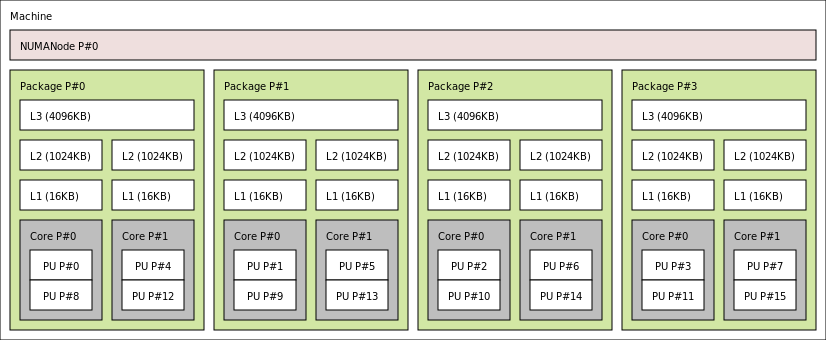
\includegraphics[width=\textwidth]{dudley.png}}
\end{DoxyImageNoCaption}


Here\textquotesingle{}s the equivalent output in textual form\+:

\begin{DoxyVerb}Machine
  NUMANode L#0 (P#0)
  Package L#0 + L3 L#0 (4096KB)
    L2 L#0 (1024KB) + L1 L#0 (16KB) + Core L#0
      PU L#0 (P#0)
      PU L#1 (P#8)
    L2 L#1 (1024KB) + L1 L#1 (16KB) + Core L#1
      PU L#2 (P#4)
      PU L#3 (P#12)
  Package L#1 + L3 L#1 (4096KB)
    L2 L#2 (1024KB) + L1 L#2 (16KB) + Core L#2
      PU L#4 (P#1)
      PU L#5 (P#9)
    L2 L#3 (1024KB) + L1 L#3 (16KB) + Core L#3
      PU L#6 (P#5)
      PU L#7 (P#13)
  Package L#2 + L3 L#2 (4096KB)
    L2 L#4 (1024KB) + L1 L#4 (16KB) + Core L#4
      PU L#8 (P#2)
      PU L#9 (P#10)
    L2 L#5 (1024KB) + L1 L#5 (16KB) + Core L#5
      PU L#10 (P#6)
      PU L#11 (P#14)
  Package L#3 + L3 L#3 (4096KB)
    L2 L#6 (1024KB) + L1 L#6 (16KB) + Core L#6
      PU L#12 (P#3)
      PU L#13 (P#11)
    L2 L#7 (1024KB) + L1 L#7 (16KB) + Core L#7
      PU L#14 (P#7)
      PU L#15 (P#15)
\end{DoxyVerb}


Note that there is also an equivalent output in X\+ML that is meant for exporting/importing topologies but it is hardly readable to human-\/beings (see \hyperlink{a00388}{Importing and exporting topologies from/to X\+ML files} for details).

On a 4-\/package 2-\/core Opteron N\+U\+MA machine (with two core cores disallowed by the administrator), the {\ttfamily lstopo} tool may show the following graphical output (with {\ttfamily -\/-\/disallowed} for displaying disallowed objects)\+:

 
\begin{DoxyImageNoCaption}
  \mbox{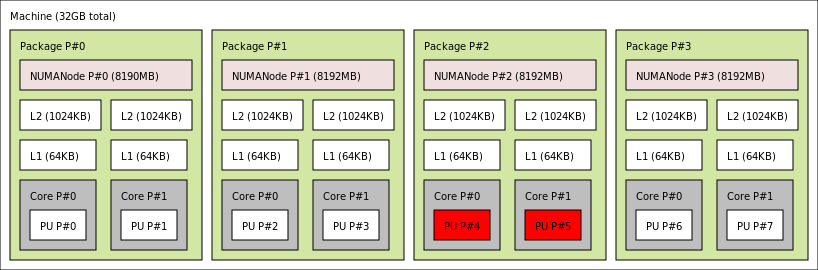
\includegraphics[width=\textwidth]{hagrid.png}}
\end{DoxyImageNoCaption}


Here\textquotesingle{}s the equivalent output in textual form\+:

\begin{DoxyVerb}Machine (32GB total)
  Package L#0
    NUMANode L#0 (P#0 8190MB)
    L2 L#0 (1024KB) + L1 L#0 (64KB) + Core L#0 + PU L#0 (P#0)
    L2 L#1 (1024KB) + L1 L#1 (64KB) + Core L#1 + PU L#1 (P#1)
  Package L#1
    NUMANode L#1 (P#1 8192MB)
    L2 L#2 (1024KB) + L1 L#2 (64KB) + Core L#2 + PU L#2 (P#2)
    L2 L#3 (1024KB) + L1 L#3 (64KB) + Core L#3 + PU L#3 (P#3)
  Package L#2
    NUMANode L#2 (P#2 8192MB)
    L2 L#4 (1024KB) + L1 L#4 (64KB) + Core L#4 + PU L#4 (P#4)
    L2 L#5 (1024KB) + L1 L#5 (64KB) + Core L#5 + PU L#5 (P#5)
  Package L#3
    NUMANode L#3 (P#3 8192MB)
    L2 L#6 (1024KB) + L1 L#6 (64KB) + Core L#6 + PU L#6 (P#6)
    L2 L#7 (1024KB) + L1 L#7 (64KB) + Core L#7 + PU L#7 (P#7)
\end{DoxyVerb}


On a 2-\/package quad-\/core Xeon (pre-\/\+Nehalem, with 2 dual-\/core dies into each package)\+:

 
\begin{DoxyImageNoCaption}
  \mbox{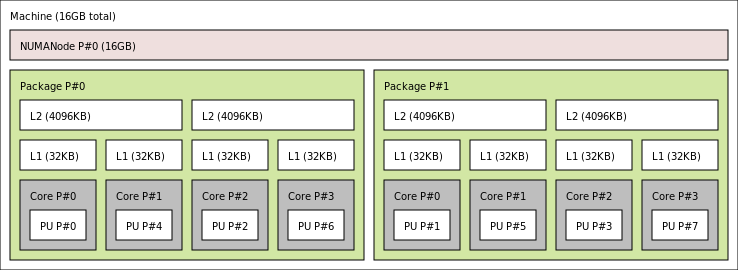
\includegraphics[width=\textwidth]{emmett.png}}
\end{DoxyImageNoCaption}


Here\textquotesingle{}s the same output in textual form\+:

\begin{DoxyVerb}Machine (total 16GB)
  NUMANode L#0 (P#0 16GB)
  Package L#0
    L2 L#0 (4096KB)
      L1 L#0 (32KB) + Core L#0 + PU L#0 (P#0)
      L1 L#1 (32KB) + Core L#1 + PU L#1 (P#4)
    L2 L#1 (4096KB)
      L1 L#2 (32KB) + Core L#2 + PU L#2 (P#2)
      L1 L#3 (32KB) + Core L#3 + PU L#3 (P#6)
  Package L#1
    L2 L#2 (4096KB)
      L1 L#4 (32KB) + Core L#4 + PU L#4 (P#1)
      L1 L#5 (32KB) + Core L#5 + PU L#5 (P#5)
    L2 L#3 (4096KB)
      L1 L#6 (32KB) + Core L#6 + PU L#6 (P#3)
      L1 L#7 (32KB) + Core L#7 + PU L#7 (P#7)
\end{DoxyVerb}


 \hypertarget{a00379_interface}{}\section{Programming Interface}\label{a00379_interface}
The basic interface is available in \hyperlink{a00119_source}{hwloc.\+h}. Some higher-\/level functions are available in \hyperlink{a00122_source}{hwloc/helper.\+h} to reduce the need to manually manipulate objects and follow links between them. Documentation for all these is provided later in this document. Developers may also want to look at hwloc/inlines.\+h which contains the actual inline code of some \hyperlink{a00119_source}{hwloc.\+h} routines, and at this document, which provides good higher-\/level topology traversal examples.

To precisely define the vocabulary used by hwloc, a \hyperlink{a00380}{Terms and Definitions} section is available and should probably be read first.

Each hwloc object contains a cpuset describing the list of processing units that it contains. These bitmaps may be used for \hyperlink{a00190}{C\+PU binding} and \hyperlink{a00191}{Memory binding}. hwloc offers an extensive bitmap manipulation interface in \hyperlink{a00125_source}{hwloc/bitmap.\+h}.

Moreover, hwloc also comes with additional helpers for interoperability with several commonly used environments. See the \hyperlink{a00390}{Interoperability With Other Software} section for details.

The complete A\+PI documentation is available in a full set of H\+T\+ML pages, man pages, and self-\/contained P\+DF files (formatted for both both US letter and A4 formats) in the source tarball in doc/doxygen-\/doc/.

{\bfseries N\+O\+TE\+:} If you are building the documentation from a Git clone, you will need to have Doxygen and pdflatex installed -- the documentation will be built during the normal \char`\"{}make\char`\"{} process. The documentation is installed during \char`\"{}make install\char`\"{} to \$prefix/share/doc/hwloc/ and your systems default man page tree (under \$prefix, of course).\hypertarget{a00379_portability}{}\subsection{Portability}\label{a00379_portability}
Operating System have varying support for C\+PU and memory binding, e.\+g. while some Operating Systems provide interfaces for all kinds of C\+PU and memory bindings, some others provide only interfaces for a limited number of kinds of C\+PU and memory binding, and some do not provide any binding interface at all. Hwloc\textquotesingle{}s binding functions would then simply return the E\+N\+O\+S\+YS error (Function not implemented), meaning that the underlying Operating System does not provide any interface for them. \hyperlink{a00190}{C\+PU binding} and \hyperlink{a00191}{Memory binding} provide more information on which hwloc binding functions should be preferred because interfaces for them are usually available on the supported Operating Systems.

Similarly, the ability of reporting topology information varies from one platform to another. As shown in \hyperlink{a00379_cli_examples}{Command-\/line Examples}, hwloc can obtain information on a wide variety of hardware topologies. However, some platforms and/or operating system versions will only report a subset of this information. For example, on an P\+P\+C64-\/based system with 8 cores (each with 2 hardware threads) running a default 2.\+6.\+18-\/based kernel from R\+H\+EL 5.\+4, hwloc is only able to glean information about N\+U\+MA nodes and processor units (P\+Us). No information about caches, packages, or cores is available.

Here\textquotesingle{}s the graphical output from lstopo on this platform when Simultaneous Multi-\/\+Threading (S\+MT) is enabled\+:

 
\begin{DoxyImageNoCaption}
  \mbox{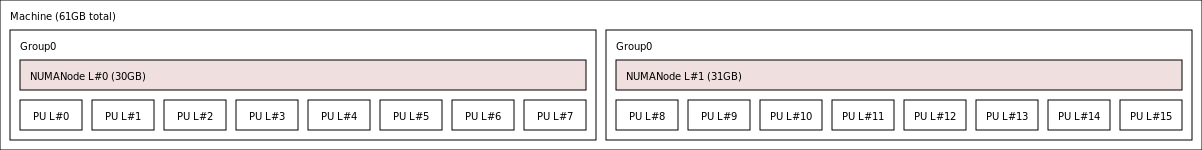
\includegraphics[width=\textwidth]{ppc64-with-smt.png}}
\end{DoxyImageNoCaption}


And here\textquotesingle{}s the graphical output from lstopo on this platform when S\+MT is disabled\+:

 
\begin{DoxyImageNoCaption}
  \mbox{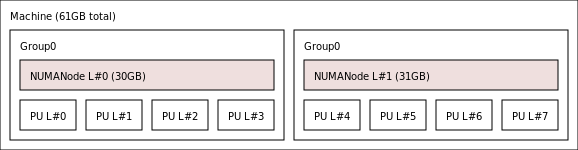
\includegraphics[width=.5\textwidth]{ppc64-without-smt.png}}
\end{DoxyImageNoCaption}


Notice that hwloc only sees half the P\+Us when S\+MT is disabled. PU L\#6, for example, seems to change location from N\+U\+MA node \#0 to \#1. In reality, no P\+Us \char`\"{}moved\char`\"{} -- they were simply re-\/numbered when hwloc only saw half as many (see also Logical index in \hyperlink{a00380_termsanddefs_indexes}{Indexes and Sets}). Hence, PU L\#6 in the S\+M\+T-\/disabled picture probably corresponds to PU L\#12 in the S\+M\+T-\/enabled picture.

This same \char`\"{}\+P\+Us have disappeared\char`\"{} effect can be seen on other platforms -- even platforms / O\+Ss that provide much more information than the above P\+P\+C64 system. This is an unfortunate side-\/effect of how operating systems report information to hwloc.

Note that upgrading the Linux kernel on the same P\+P\+C64 system mentioned above to 2.\+6.\+34, hwloc is able to discover all the topology information. The following picture shows the entire topology layout when S\+MT is enabled\+:

 
\begin{DoxyImageNoCaption}
  \mbox{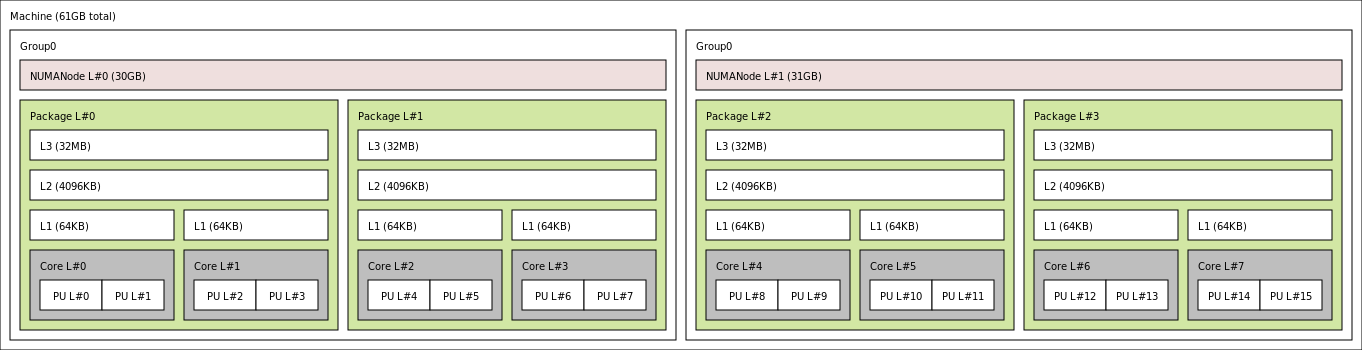
\includegraphics[width=\textwidth]{ppc64-full-with-smt.png}}
\end{DoxyImageNoCaption}


Developers using the hwloc A\+PI or X\+ML output for portable applications should therefore be extremely careful to not make any assumptions about the structure of data that is returned. For example, per the above reported P\+PC topology, it is not safe to assume that P\+Us will always be descendants of cores.

Additionally, future hardware may insert new topology elements that are not available in this version of hwloc. Long-\/lived applications that are meant to span multiple different hardware platforms should also be careful about making structure assumptions. For example, a new element may someday exist between a core and a PU.\hypertarget{a00379_interface_example}{}\subsection{A\+P\+I Example}\label{a00379_interface_example}
The following small C example (available in the source tree as ``doc/examples/hwloc-\/hello.c\textquotesingle{}\textquotesingle{}) prints the topology of the machine and performs some thread and memory binding. More examples are available in the doc/examples/ directory of the source tree.


\begin{DoxyCodeInclude}
\textcolor{comment}{/* Example hwloc API program.}
\textcolor{comment}{ *}
\textcolor{comment}{ * See other examples under doc/examples/ in the source tree}
\textcolor{comment}{ * for more details.}
\textcolor{comment}{ *}
\textcolor{comment}{ * Copyright © 2009-2016 Inria.  All rights reserved.}
\textcolor{comment}{ * Copyright © 2009-2011 Université Bordeaux}
\textcolor{comment}{ * Copyright © 2009-2010 Cisco Systems, Inc.  All rights reserved.}
\textcolor{comment}{ * See COPYING in top-level directory.}
\textcolor{comment}{ *}
\textcolor{comment}{ * hwloc-hello.c}
\textcolor{comment}{ */}

\textcolor{preprocessor}{#include "hwloc.h"}

\textcolor{preprocessor}{#include <errno.h>}
\textcolor{preprocessor}{#include <stdio.h>}
\textcolor{preprocessor}{#include <string.h>}

\textcolor{keyword}{static} \textcolor{keywordtype}{void} print\_children(\hyperlink{a00186_ga9d1e76ee15a7dee158b786c30b6a6e38}{hwloc\_topology\_t} topology, 
      \hyperlink{a00238}{hwloc\_obj\_t} obj,
                           \textcolor{keywordtype}{int} depth)
\{
    \textcolor{keywordtype}{char} type[32], attr[1024];
    \textcolor{keywordtype}{unsigned} i;

    \hyperlink{a00188_gadb8765c260edea80c52cd06a76639ba4}{hwloc\_obj\_type\_snprintf}(type, \textcolor{keyword}{sizeof}(type), obj, 0);
    printf(\textcolor{stringliteral}{"%*s%s"}, 2*depth, \textcolor{stringliteral}{""}, type);
    \textcolor{keywordflow}{if} (obj->\hyperlink{a00238_a61a7a80a68eaccbaaa28269e678c81a9}{os\_index} != (\textcolor{keywordtype}{unsigned}) -1)
      printf(\textcolor{stringliteral}{"#%u"}, obj->\hyperlink{a00238_a61a7a80a68eaccbaaa28269e678c81a9}{os\_index});
    \hyperlink{a00188_ga870e876931c282a1c7aee2f031912ce3}{hwloc\_obj\_attr\_snprintf}(attr, \textcolor{keyword}{sizeof}(attr), obj, \textcolor{stringliteral}{" "}, 0);
    \textcolor{keywordflow}{if} (*attr)
      printf(\textcolor{stringliteral}{"(%s)"}, attr);
    printf(\textcolor{stringliteral}{"\(\backslash\)n"});
    \textcolor{keywordflow}{for} (i = 0; i < obj->\hyperlink{a00238_aac3f6da35c9b57599909a44ce2b716c1}{arity}; i++) \{
        print\_children(topology, obj->\hyperlink{a00238_a04d05403da37bfe17cd63b7c7dd07b1f}{children}[i], depth + 1);
    \}
\}

\textcolor{keywordtype}{int} main(\textcolor{keywordtype}{void})
\{
    \textcolor{keywordtype}{int} \hyperlink{a00238_a4876fd165b4fff35521f07ebd85355ed}{depth};
    \textcolor{keywordtype}{unsigned} i, n;
    \textcolor{keywordtype}{unsigned} \textcolor{keywordtype}{long} size;
    \textcolor{keywordtype}{int} levels;
    \textcolor{keywordtype}{char} \textcolor{keywordtype}{string}[128];
    \textcolor{keywordtype}{int} topodepth;
    \textcolor{keywordtype}{void} *m;
    \hyperlink{a00186_ga9d1e76ee15a7dee158b786c30b6a6e38}{hwloc\_topology\_t} topology;
    \hyperlink{a00183_ga4bbf39b68b6f568fb92739e7c0ea7801}{hwloc\_cpuset\_t} \hyperlink{a00238_a67925e0f2c47f50408fbdb9bddd0790f}{cpuset};
    \hyperlink{a00238}{hwloc\_obj\_t} obj;

    \textcolor{comment}{/* Allocate and initialize topology object. */}
    \hyperlink{a00186_ga03fd4a16d8b9ee1ffc32b25fd2f6bdfa}{hwloc\_topology\_init}(&topology);

    \textcolor{comment}{/* ... Optionally, put detection configuration here to ignore}
\textcolor{comment}{       some objects types, define a synthetic topology, etc....}
\textcolor{comment}{}
\textcolor{comment}{       The default is to detect all the objects of the machine that}
\textcolor{comment}{       the caller is allowed to access.  See Configure Topology}
\textcolor{comment}{       Detection. */}

    \textcolor{comment}{/* Perform the topology detection. */}
    \hyperlink{a00186_gabdf58d87ad77f6615fccdfe0535ff826}{hwloc\_topology\_load}(topology);

    \textcolor{comment}{/* Optionally, get some additional topology information}
\textcolor{comment}{       in case we need the topology depth later. */}
    topodepth = \hyperlink{a00187_gae54d1782ca9b54bea915f5c18a9158fa}{hwloc\_topology\_get\_depth}(topology);

    \textcolor{comment}{/*****************************************************************}
\textcolor{comment}{     * First example:}
\textcolor{comment}{     * Walk the topology with an array style, from level 0 (always}
\textcolor{comment}{     * the system level) to the lowest level (always the proc level).}
\textcolor{comment}{     *****************************************************************/}
    \textcolor{keywordflow}{for} (depth = 0; depth < topodepth; depth++) \{
        printf(\textcolor{stringliteral}{"*** Objects at level %d\(\backslash\)n"}, depth);
        \textcolor{keywordflow}{for} (i = 0; i < \hyperlink{a00187_ga1d5ceafe8130fe6e8657bf0bc666ba50}{hwloc\_get\_nbobjs\_by\_depth}(topology, depth);
             i++) \{
            \hyperlink{a00188_gadb8765c260edea80c52cd06a76639ba4}{hwloc\_obj\_type\_snprintf}(\textcolor{keywordtype}{string}, \textcolor{keyword}{sizeof}(\textcolor{keywordtype}{string}),
                                    \hyperlink{a00187_ga391f6b2613f0065673eaa4069b93d4e0}{hwloc\_get\_obj\_by\_depth}(topology, depth, i), 0);
            printf(\textcolor{stringliteral}{"Index %u: %s\(\backslash\)n"}, i, \textcolor{keywordtype}{string});
        \}
    \}

    \textcolor{comment}{/*****************************************************************}
\textcolor{comment}{     * Second example:}
\textcolor{comment}{     * Walk the topology with a tree style.}
\textcolor{comment}{     *****************************************************************/}
    printf(\textcolor{stringliteral}{"*** Printing overall tree\(\backslash\)n"});
    print\_children(topology, \hyperlink{a00187_ga2d4b12fc187dfc53b35f2fa21d21044d}{hwloc\_get\_root\_obj}(topology), 0);

    \textcolor{comment}{/*****************************************************************}
\textcolor{comment}{     * Third example:}
\textcolor{comment}{     * Print the number of packages.}
\textcolor{comment}{     *****************************************************************/}
    depth = \hyperlink{a00187_ga8bec782e21be313750da70cf7428b374}{hwloc\_get\_type\_depth}(topology, \hyperlink{a00184_ggacd37bb612667dc437d66bfb175a8dc55ab16ab8c0dbffc234921d86f3dfb63129}{HWLOC\_OBJ\_PACKAGE});
    \textcolor{keywordflow}{if} (depth == \hyperlink{a00187_ggaf4e663cf42bbe20756b849c6293ef575a0565ab92ab72cb0cec91e23003294aad}{HWLOC\_TYPE\_DEPTH\_UNKNOWN}) \{
        printf(\textcolor{stringliteral}{"*** The number of packages is unknown\(\backslash\)n"});
    \} \textcolor{keywordflow}{else} \{
        printf(\textcolor{stringliteral}{"*** %u package(s)\(\backslash\)n"},
               \hyperlink{a00187_ga1d5ceafe8130fe6e8657bf0bc666ba50}{hwloc\_get\_nbobjs\_by\_depth}(topology, depth));
    \}

    \textcolor{comment}{/*****************************************************************}
\textcolor{comment}{     * Fourth example:}
\textcolor{comment}{     * Compute the amount of cache that the first logical processor}
\textcolor{comment}{     * has above it.}
\textcolor{comment}{     *****************************************************************/}
    levels = 0;
    size = 0;
    \textcolor{keywordflow}{for} (obj = \hyperlink{a00187_ga6f414dd80a2b943967a0ac92da3181a2}{hwloc\_get\_obj\_by\_type}(topology, \hyperlink{a00184_ggacd37bb612667dc437d66bfb175a8dc55abca6887e80cb291353b0a0c1da83f661}{HWLOC\_OBJ\_PU}, 0);
         obj;
         obj = obj->\hyperlink{a00238_adc494f6aed939992be1c55cca5822900}{parent})
      \textcolor{keywordflow}{if} (\hyperlink{a00198_ga2ed589bea28711e80b92066510a5607d}{hwloc\_obj\_type\_is\_cache}(obj->\hyperlink{a00238_acc4f0803f244867e68fe0036800be5de}{type})) \{
        levels++;
        size += obj->\hyperlink{a00238_accd40e29f71f19e88db62ea3df02adc8}{attr}->\hyperlink{a00242_ab5a8ae3bf490e6b1071fea53f7382836}{cache}.\hyperlink{a00254_abe5e788943ed04302976740c829674c0}{size};
      \}
    printf(\textcolor{stringliteral}{"*** Logical processor 0 has %d caches totaling %luKB\(\backslash\)n"},
           levels, size / 1024);

    \textcolor{comment}{/*****************************************************************}
\textcolor{comment}{     * Fifth example:}
\textcolor{comment}{     * Bind to only one thread of the last core of the machine.}
\textcolor{comment}{     *}
\textcolor{comment}{     * First find out where cores are, or else smaller sets of CPUs if}
\textcolor{comment}{     * the OS doesn't have the notion of a "core".}
\textcolor{comment}{     *****************************************************************/}
    depth = \hyperlink{a00187_ga8125328e69eba709c33ea8055c12589b}{hwloc\_get\_type\_or\_below\_depth}(topology, 
      \hyperlink{a00184_ggacd37bb612667dc437d66bfb175a8dc55ac793958f330bca371aa1535de8aff45f}{HWLOC\_OBJ\_CORE});

    \textcolor{comment}{/* Get last core. */}
    obj = \hyperlink{a00187_ga391f6b2613f0065673eaa4069b93d4e0}{hwloc\_get\_obj\_by\_depth}(topology, depth,
                   \hyperlink{a00187_ga1d5ceafe8130fe6e8657bf0bc666ba50}{hwloc\_get\_nbobjs\_by\_depth}(topology, depth) - 1);
    \textcolor{keywordflow}{if} (obj) \{
        \textcolor{comment}{/* Get a copy of its cpuset that we may modify. */}
        cpuset = \hyperlink{a00205_gae679434c1a5f41d3560a8a7e2c1b0dee}{hwloc\_bitmap\_dup}(obj->\hyperlink{a00238_a67925e0f2c47f50408fbdb9bddd0790f}{cpuset});

        \textcolor{comment}{/* Get only one logical processor (in case the core is}
\textcolor{comment}{           SMT/hyper-threaded). */}
        \hyperlink{a00205_gaa611a77c092e679246afdf9a60d5db8b}{hwloc\_bitmap\_singlify}(cpuset);

        \textcolor{comment}{/* And try to bind ourself there. */}
        \textcolor{keywordflow}{if} (\hyperlink{a00190_ga80bc07473a8edf840cae17bd7ec21d48}{hwloc\_set\_cpubind}(topology, cpuset, 0)) \{
            \textcolor{keywordtype}{char} *str;
            \textcolor{keywordtype}{int} error = errno;
            \hyperlink{a00205_ga0fece972134fdecf2da9bc7a11dd827e}{hwloc\_bitmap\_asprintf}(&str, obj->\hyperlink{a00238_a67925e0f2c47f50408fbdb9bddd0790f}{cpuset});
            printf(\textcolor{stringliteral}{"Couldn't bind to cpuset %s: %s\(\backslash\)n"}, str, strerror(error));
            free(str);
        \}

        \textcolor{comment}{/* Free our cpuset copy */}
        \hyperlink{a00205_ga156130d85b3a0674d6e0e6770fe68fbe}{hwloc\_bitmap\_free}(cpuset);
    \}

    \textcolor{comment}{/*****************************************************************}
\textcolor{comment}{     * Sixth example:}
\textcolor{comment}{     * Allocate some memory on the last NUMA node, bind some existing}
\textcolor{comment}{     * memory to the last NUMA node.}
\textcolor{comment}{     *****************************************************************/}
    \textcolor{comment}{/* Get last node. There's always at least one. */}
    n = \hyperlink{a00187_ga789a3f65aedff644be64a18526a03065}{hwloc\_get\_nbobjs\_by\_type}(topology, 
      \hyperlink{a00184_ggacd37bb612667dc437d66bfb175a8dc55a9d917a3e5497950c6d8948b8e183db5a}{HWLOC\_OBJ\_NUMANODE});
    obj = \hyperlink{a00187_ga6f414dd80a2b943967a0ac92da3181a2}{hwloc\_get\_obj\_by\_type}(topology, 
      \hyperlink{a00184_ggacd37bb612667dc437d66bfb175a8dc55a9d917a3e5497950c6d8948b8e183db5a}{HWLOC\_OBJ\_NUMANODE}, n - 1);

    size = 1024*1024;
    m = \hyperlink{a00191_ga04736461780fadcf193af218c0122273}{hwloc\_alloc\_membind}(topology, size, obj->\hyperlink{a00238_a08f0d0e16c619a6e653526cbee4ffea3}{nodeset},
                            \hyperlink{a00191_ggac9764f79505775d06407b40f5e4661e8ad811fa4b2a6002c4d63695a408ffde2c}{HWLOC\_MEMBIND\_BIND}, 
      \hyperlink{a00191_ggab00475fd98815bf4fb9aaf752030e7d2a71f19fe4505f1c083dc8e6f7bdea6256}{HWLOC\_MEMBIND\_BYNODESET});
    \hyperlink{a00191_ga32dbd4f54e9e4a7179f2dde37ffe6ad7}{hwloc\_free}(topology, m, size);

    m = malloc(size);
    \hyperlink{a00191_gaf881faefe20701229f07dd7dbd0125ed}{hwloc\_set\_area\_membind}(topology, m, size, obj->\hyperlink{a00238_a08f0d0e16c619a6e653526cbee4ffea3}{nodeset},
                           \hyperlink{a00191_ggac9764f79505775d06407b40f5e4661e8ad811fa4b2a6002c4d63695a408ffde2c}{HWLOC\_MEMBIND\_BIND}, 
      \hyperlink{a00191_ggab00475fd98815bf4fb9aaf752030e7d2a71f19fe4505f1c083dc8e6f7bdea6256}{HWLOC\_MEMBIND\_BYNODESET});
    free(m);

    \textcolor{comment}{/* Destroy topology object. */}
    \hyperlink{a00186_ga9f34a640b6fd28d23699d4d084667b15}{hwloc\_topology\_destroy}(topology);

    \textcolor{keywordflow}{return} 0;
\}
\end{DoxyCodeInclude}


hwloc provides a {\ttfamily pkg-\/config} executable to obtain relevant compiler and linker flags. For example, it can be used thusly to compile applications that utilize the hwloc library (assuming G\+NU Make)\+:

\begin{DoxyVerb}CFLAGS += $(shell pkg-config --cflags hwloc)
LDLIBS += $(shell pkg-config --libs hwloc)

hwloc-hello: hwloc-hello.c
        $(CC) hwloc-hello.c $(CFLAGS) -o hwloc-hello $(LDLIBS)
\end{DoxyVerb}


On a machine 2 processor packages -- each package of which has two processing cores -- the output from running {\ttfamily hwloc-\/hello} could be something like the following\+:

\begin{DoxyVerb}shell$ ./hwloc-hello
*** Objects at level 0
Index 0: Machine
*** Objects at level 1
Index 0: Package#0
Index 1: Package#1
*** Objects at level 2
Index 0: Core#0
Index 1: Core#1
Index 2: Core#3
Index 3: Core#2
*** Objects at level 3
Index 0: PU#0
Index 1: PU#1
Index 2: PU#2
Index 3: PU#3
*** Printing overall tree
Machine
  Package#0
    Core#0
      PU#0
    Core#1
      PU#1
  Package#1
    Core#3
      PU#2
    Core#2
      PU#3
*** 2 package(s)
*** Logical processor 0 has 0 caches totaling 0KB
shell$ 
\end{DoxyVerb}


 \hypertarget{a00379_history}{}\section{History / Credits}\label{a00379_history}
hwloc is the evolution and merger of the libtopology project and the Portable Linux Processor Affinity (P\+L\+PA) (\href{https://www.open-mpi.org/projects/plpa/}{\tt https\+://www.\+open-\/mpi.\+org/projects/plpa/}) project. Because of functional and ideological overlap, these two code bases and ideas were merged and released under the name \char`\"{}hwloc\char`\"{} as an Open M\+PI sub-\/project.

libtopology was initially developed by the Inria Runtime Team-\/\+Project. P\+L\+PA was initially developed by the Open M\+PI development team as a sub-\/project. Both are now deprecated in favor of hwloc, which is distributed as an Open M\+PI sub-\/project.

 \hypertarget{a00379_further_reading}{}\section{Further Reading}\label{a00379_further_reading}
The documentation chapters include


\begin{DoxyItemize}
\item \hyperlink{a00380}{Terms and Definitions} 
\item \hyperlink{a00381}{Command-\/\+Line Tools} 
\item \hyperlink{a00382}{Environment Variables} 
\item \hyperlink{a00383}{C\+PU and Memory Binding Overview} 
\item \hyperlink{a00384}{I/O Devices} 
\item \hyperlink{a00385}{Miscellaneous objects} 
\item \hyperlink{a00386}{Object attributes} 
\item \hyperlink{a00387}{Topology Attributes\+: Distances, Memory Attributes and C\+PU Kinds} 
\item \hyperlink{a00388}{Importing and exporting topologies from/to X\+ML files} 
\item \hyperlink{a00389}{Synthetic topologies} 
\item \hyperlink{a00390}{Interoperability With Other Software} 
\item \hyperlink{a00391}{Thread Safety} 
\item \hyperlink{a00392}{Components and plugins} 
\item \hyperlink{a00393}{Embedding hwloc in Other Software} 
\item \hyperlink{a00394}{Frequently Asked Questions} 
\item \hyperlink{a00395}{Upgrading to the hwloc 2.\+0 A\+PI} 
\end{DoxyItemize}

Make sure to have had a look at those too!

 